\DocumentMetadata{
	lang=zh-CN,
	pdfversion=2.0,
	pdfstandard=A-4,
	tagging=on
}
\documentclass{article}

\title{读螺旋式曲线开沟混肥装置有机肥排肥防堵结构设计与试验}
\author{石成玉}
\date{\today}

\usepackage{amsmath}
\usepackage{geometry}
\usepackage{float}
\usepackage{tikz}
\usepackage{hyperref}
\usepackage{fancyhdr}
\usepackage{graphics}
\usepackage{booktabs}
\usepackage{tcolorbox}
\usepackage{ctex}

\pdfvariable minorversion=7

\geometry{hmargin=1in,vmargin=1in,a4paper}

\makeatletter
\hypersetup{
	colorlinks,
	linkcolor=blue,
	pdfencoding=auto,
	pdftitle={\@title},
	pdfauthor={\@author},
	pdfcreator=LaTeX
}
\makeatother

\tcbset{
	before upper={\parindent2em}
}

\usetikzlibrary{graphdrawing,graphs,arrows.meta}
\usegdlibrary{layered}

\begin{document}
	
\maketitle

\tableofcontents

\section{论文关系}

解决了\href{https://doi.org/10.27409/d.cnki.gxbnu.2020.000732}{矮砧果园有机肥料开沟施肥装置设计与试验\_臧家俊}中,有机肥堵塞的问题。

\section{研究背景和意义}

\subsection{为什么要研究?}

\begin{figure}[H]
	\centering
	\begin{tikzpicture}[nodes={draw=black,thick},rounded corners]
		\graph[layered layout] {
		"中国水果的国际竞争力低"->"同矮砧种植技术果品不如外国"->"土壤有机质含量偏低"->{"果园土壤有机质含量偏低","化学肥料的过度使用"}->"有机质含量影响果品"->"施有机肥"->"课题组先前施肥机存在堵塞问题"->"解决堵塞问题";
		};
	\end{tikzpicture}
\end{figure}

\begin{enumerate}
	\item 我国是水果生产大国,却不是水果生产强国;国际影响力弱、竞争力弱行业标准水平低;生产高品优质水果对我国水果产业发展意义重大。
	\item 同样采用矮砧密植,我国苹果单产及果品品质较国外一些国家仍具有明显差距,造成这一现象的原因很大程度上与果树生长的土壤环境以及果树对养分的吸收有关。
	\item 土壤是果树生长的重要载体,土壤有机质是土壤固相的重要组成部分,是直接决定土壤肥力的物质基础。而我国果园土壤有机质含量普遍偏低。因此,土壤有机质含量低已经成为了制约我国水果产业可持续发展的重要原因。
	\item 我国水果产业单产产量及果品品质偏低的另一重要原因是化学肥料的过度使用。因此,减少化学肥料施用,采用科学合理的施肥技术,已成为我国水果产业提质增效和可持续发展的重要途径。
	\item 土壤有机质在果树优质高效生产中具有重要作用,提高果园有机质含量不仅能实现稳产高产,还能提高果品品质。
	\item 果园环状沟施肥是果树最为理想的施肥方式。然而,在现有研究阶段,可适用于果园环沟施肥方式的有机肥开沟施肥装备仍处于空白,高效施肥装备的缺门断档成为了制约我国水果产业高效发展的瓶颈问题。
	\item 本课题组先前的施肥机\href{https://doi.org/10.27409/d.cnki.gxbnu.2020.000732}{矮砧果园有机肥料开沟施肥装置设计与试验\_臧家俊}存在肥料堵塞的问题。
\end{enumerate}

\subsection{解决了什么问题?}

\begin{enumerate}
	\item 螺旋式曲线开沟混肥装置高速旋转的排肥管内有机肥堵塞机理尚不清楚的。
	\item 设计螺旋式曲线开沟混肥装置有机肥排肥防堵结构。
	\item 通过离散元仿真研究对防堵结构进一步优化设计,探究防堵结构对排肥性能的影响机制和施肥作业过程中排肥性能改变对肥-土混合性能的影响。
\end{enumerate}

\section{存在的问题}

\subsection{仿真结果云图图例不合适}

\begin{tcolorbox}
	\begin{figure}[H]
		\centering
		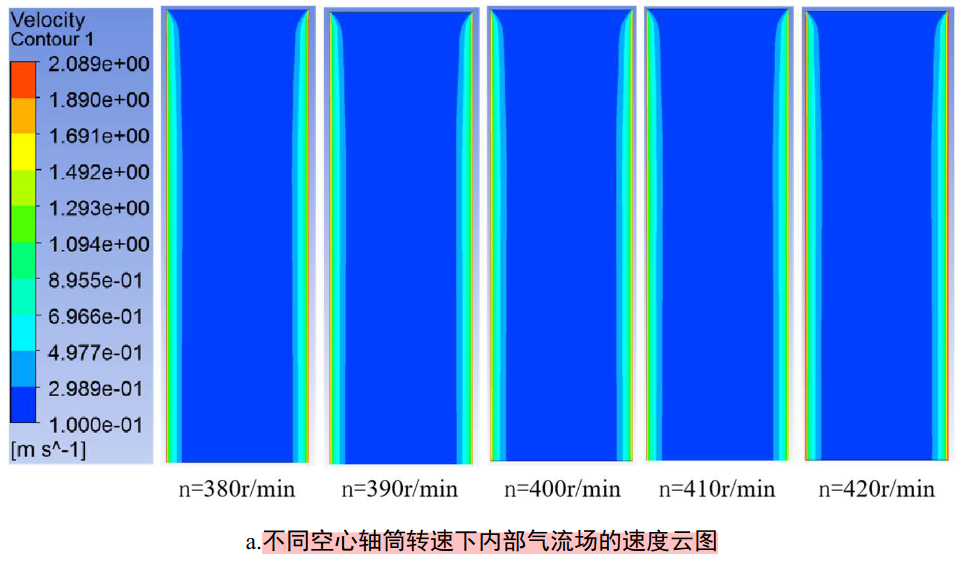
\includegraphics[width=0.5\textwidth]{../assets/不同空心轴筒转速下内部气流场的速度云图.png}
		\caption{不同空心轴筒转速下内部气流场的结果云图}
	\end{figure}
	\raggedleft{\href{https://doi.org/10.27409/d.cnki.gxbnu.2020.000732}{——Page.21 矮砧果园有机肥料开沟施肥装置设计与试验\_臧家俊}}
\end{tcolorbox}

\subsection{似乎有前后矛盾}

\begin{tcolorbox}
	2.2.3.6 空心轴筒前进速度对有机肥排肥性能的影响规律
	
	空心轴筒运动状态下,其前进速度对有机肥排肥性能几乎没有影响。随着空心轴筒前进速度的增加,有机肥在空心轴筒内壁上的粘附量(4688、4726、4716、4657、4732)几乎没有变化。
	
	2.2.4 传动箱空心轴筒内壁堵肥分析总结
	
	同时,本节研究了传动箱空心轴筒运动状态下对有机肥排肥性能的影响。随着空心轴筒前进速度的增加,有机肥在空心轴筒内壁上的粘附量逐渐增多,有机肥排肥性能逐渐变差。当空心轴筒的前进速度小于0.28m/s(即1km/h)时,有机肥在筒壁上的粘附量小于空心轴筒静止状态下有机肥的粘附量;而当空心轴筒的前进速度大于0.28m/s时,有机肥在筒壁上的粘附量才有了显著的增加。这说明空心轴筒具有一定前进速度的情况下,可以减少有机肥与壁面之间的粘附作用。
	
	\raggedleft{\href{https://doi.org/10.27409/d.cnki.gxbnu.2020.000732}{——Page.35 矮砧果园有机肥料开沟施肥装置设计与试验\_臧家俊}}
\end{tcolorbox}

\subsection{为什么}

\begin{tcolorbox}
	当螺旋叶片的转速大于其临界转速时,螺旋叶片转速越大,其对土壤的提升作用越强,开沟混肥器开沟前进过程中,受前方土壤阻碍作用,出肥口下方的螺旋叶片提升的土壤会阻碍出肥口排肥,进而减低了开沟混肥器的排肥速率,对开沟混肥器的排肥性能具有不利影响。因此必须对开沟混肥器的入土结构进行改进,在保证其入土性能的基础上,减小其对土壤的提升作用,进而使得开沟混肥器的有机肥排肥速率提高,从而提高开沟混肥器的有机肥排肥性能,避免发生有机肥堵肥问题。
	
	\raggedleft{\href{https://doi.org/10.27409/d.cnki.gxbnu.2020.000732}{——Page.38 矮砧果园有机肥料开沟施肥装置设计与试验\_臧家俊}}
\end{tcolorbox}

\section{一些想法}

\subsection{关于开沟器圆筒的形状设计}

\textbf{是否可以将圆筒内腔设计为圆锥形?}

将圆筒内腔设计为下方直径大,上方直径小的圆锥形。在圆筒旋转时,有机肥粒受到的来自圆筒内壁的反力就可以分解出一个向下的力。

\section{研究过程}

\subsection{堵塞原因分析}

\subsubsection{EDEM-FLUENT耦合仿真}

\begin{description}
	\item[EDEM-Fluent耦合仿真]
	
	EDEM-Fluent耦合过程是一个瞬态双向数据传递的过程。首先,利用Fluent计算一个时间步的流场信息,然后启动EDEM进行相同时间迭代,利用耦合接口将颗粒的位置、运动、体积、温度等信息传递至Fluent中,计算颗粒与流体的相互作用,流体对颗粒的作用将通过接口传递至EDEM作为颗粒体积力影响颗粒的运动,而对流体的作用通过动量源相的方式作用于流体中。逐步循环迭代,实现全过程的瞬态模拟。
\end{description}

通过控制变量的单因素仿真试验,确定了空心轴筒转速、直径和前进速度对有机肥粘附情况的影响规律。

\subsubsection{前进时排肥口有“吃土”现象}

在施肥机前进过程中,由于排肥会旋转至朝向前进方向,产生土壤阻挡甚至进入排肥口的现象,导致排肥不畅和堵塞。

\end{document}